\documentclass{ltjsbook}%
\usepackage{amssymb}%
\usepackage{amsthm}%
\usepackage{eulervm}%
\usepackage[%
  twoside,%
  paperwidth = 188mm,%
  paperheight = 263mm,%
  layoutwidth = 182mm,%
  layoutheight = 257mm,%
  layouthoffset = 3mm,%
  layoutvoffset = 3mm,%
  textwidth = 160mm,%
  textheight = 240mm,%
  left = 11mm,%
  right = 11mm,%
  top = 17mm,%
  bottom = 10mm,%
  headheight = 5mm,%
  headsep = 6mm%
]{geometry}%
\usepackage{luatexja-fontspec}%
\usepackage{mathtools}%
\usepackage{proof}%
\usepackage{tikz}%
\usepackage{titlesec}%
\usepackage{titletoc}%
\usepackage{xpatch}%
% amsthm
\renewcommand\proofname{証明}%
\newtheorem{theorem}{定理}[section]%
\newtheorem{lemma}{補題}[section]%
\newtheorem{example}{例}[section]%
% luatexja-fontspec
\setmainfont{Novelty Light}%
\setsansfont{Novelty Light}%
\setmonofont{Journal}%
\setmainjfont{CandGReithic04}%
\setsansjfont{CandGReithic04}%
\newfontfamily\ebgaramond{EB Garamond}%
\newfontfamily\news{C4_News_R}%
\newjfontfamily\sbnreim{vsbmitaM}%
\newfontfamily\terra{Terra Narrow}%
% mathtools
\mathtoolsset{showonlyrefs = true}%
% tikz
\usetikzlibrary{arrows}%
\usetikzlibrary{lindenmayersystems}%
\pgfdeclarelindenmayersystem{Hilbert curve}{%
  \rule{L -> +RF-LFL-FR+}%
  \rule{R -> -LF+RFR+FL-}}%
% titlesec
\newpagestyle{techbookfest}{%
  \sethead[%
    {\ebgaramond\textit{\thepage}}][][]{}{}{%
    {\ebgaramond\textit{\thepage}}}%
  \setfoot[][][]{}{}{}}%
\assignpagestyle{\chapter}{techbookfest}%
\xpretocmd\chapter{\pagestyle{techbookfest}}{}{}%
\titleformat{\chapter}[block]{\Large\centering}{%
  \prechaptername\thechapter\postchaptername\quad}{0mm}{}%
\titleformat{\section}[block]{§\thesection.\quad}{}{0mm}{}%
% titletoc
\titlecontents{chapter}[5\zw]{%
  %\addvspace{1\zh}
  \contentslabel[{\thecontentslabel}]{5\zw}}{}{}{%
  \normalsize\hspace*{\fill}{\ebgaramond{\textit{\contentspage}}}}%
\titlecontents{section}[6\zw]{\contentslabel[%
    \S\thecontentslabel.]{6\zw}}{}{}{%
  \normalsize\titlerule*[1.5mm]{.}{\ebgaramond{\textit{\contentspage}}}}%
% personal commands
\newcommand\lemmaname{補題}%
\newcommand\term[2]{\textbf{#1}{(\textit{#2})}}%
\newlength\logowidth%
\settowidth\logowidth{\terra\Large An Introduction to Lambda Calculus}%
\begin{document}%
\pagestyle{empty}%
\begin{tikzpicture}[remember picture, overlay]%
  \node [%
    minimum width = 686.0086mm,%
    minimum height = 263.0043mm%
  ] at (current page.center) {%
    \begin{minipage}[t][263.0043mm]{686.0086mm}%
      \begin{flushright}%
        \begin{minipage}[t][263.0043mm]{263.0043mm}%
          \begin{tikzpicture}%
            \shadedraw%
              [bottom color=white, top color=white, draw=black, thick]%
              [l-system =%
                {Hilbert curve, axiom=L, order=7, step=2.0709mm, angle=90}]%
              lindenmayer system;%
          \end{tikzpicture}%
        \end{minipage}%
      \end{flushright}%
    \end{minipage}};%
\end{tikzpicture}%
\begin{tikzpicture}[remember picture, overlay]%
  \node [%
    minimum width = \paperwidth,%
    minimum height = \paperheight%
  ] at (current page.center) {%
    \begin{minipage}[t][\textheight]{\textwidth}%
      \vspace*{55.27864mm}%
      \hspace*{\the\dimexpr(\logowidth-0.25\textwidth)/2\relax}%
      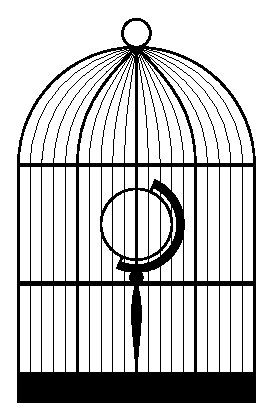
\includegraphics{logo.eps}%
    \end{minipage}};%
\end{tikzpicture}%
\begin{tikzpicture}[remember picture, overlay]%
  \node [%
    minimum width = \paperwidth,%
    minimum height = \paperheight%
  ] at (current page.center) {%
    \begin{minipage}[t][\textheight]{\textwidth}%
      \vspace*{0.5\textheight}%
      \begin{minipage}[t][0.125\textheight]{\textwidth}%
        \begin{minipage}[t][10mm]{\the\logowidth}%
          \vfill%
          {\terra\small\textit{Wir müssen wissen. Wir werden wissen.}}%
        \end{minipage}%
        \vfill%
        \begin{minipage}[t][15mm]{\the\logowidth}%
          \vspace*{\fill}%
          {\terra\Large An Introduction to Lambda Calculus}%
          {\news\scriptsize ラ\hspace*{\fill}ム\hspace*{\fill}ダ\hspace*{\fill}%
            計\hspace*{\fill}算\hspace*{\fill}入\hspace*{\fill}門}%
          \vspace*{\fill}%
        \end{minipage}%
        \vfill%
        \begin{minipage}[t][10mm]{\the\logowidth}%
          \hfill%
          {\sbnreim 川向薫}%
        \end{minipage}%
      \end{minipage}%
    \end{minipage}};%
\end{tikzpicture}%
\cleardoublepage%
\let\originalcleardoublepage\cleardoublepage%
\let\cleardoublepage\clearpage%
%\pagestyle{techbookfest}%
\frontmatter%
\chapter{はしがき}%
\hspace*{1\zw}本書はひとつのラムダ計算の入門書です.%
\prechaptername\ref{chap:untyped}\postchaptername では%
型なしラムダ計算を扱い, \prechaptername\ref{chap:typed}\postchaptername では%
単純型つきラムダ計算を扱いまして,%
\prechaptername\ref{chap:infer}\postchaptername では%
単純型つきラムダ計算の型推論を扱います.%
\iffalse%
本書は集合論や述語論理の知識を仮定しています.%
本書の証明は述語論理の言葉で書かれています.%
たとえば$a=b$かつ$b=c$かつ$c=d$という前提のもとで$a=d$を証明する場合,%
\begin{enumerate}%
\item 前提: $a=b$
\item 前提: $b=c$
\item 前提: $c=d$
\item 1, 2 より $a=c$
\item 3, 4 より $a=d$
\end{enumerate}%
などと書く代わりに%
\begin{equation}%
  \infer{%
    a=b,b=c,c=d\vdash a=d%
  }{%
    \infer{%
      a=b,b=c\vdash a=c%
    }{%
      a=b\vdash a=b%
    &%
      b=c\vdash b=c%
    }%
  &%
    c=d\vdash d=d%
  }%
\end{equation}%
というように書くのです.%
$\vdash$の左側は仮定の列で,右側は命題です.%
横線は割り算ではなく,なんらかの推論規則------この場合は推移律------を%
表しているのです.厳密には述語論理には通常,``=''という記号が含まれていません%
ので述語論理を``通常の数学の言葉''で拡張した体系で証明を書くことになります.%
つまり通常の述語論理の推論規則に加えて通常の数学の公理や推論は%
いちいち説明せずに使うということです.%
とはいえなんの説明もなしにというのも不親切ですので,%
よく使う推論規則はここに示しておきます.%
とくにつぎのみっつの------それぞれ\term{弱化}{weakening},%
\term{縮約}{contraction},\term{交換}{exchanging}と呼ばれる------推論規則%
については,簡単のため常に認められるものとしています.%
\begin{equation}%
  \infer{%
    \Gamma,\alpha\vdash \beta%
  }{%
    \Gamma\vdash\beta%
  }%
\end{equation}%
\begin{equation}%
  \infer{%
    \Gamma,\alpha,\alpha\vdash\beta%
  }{%
    \Gamma,\alpha\vdash\beta%
  }%
\end{equation}%
\begin{equation}%
  \infer{%
    \Gamma,\alpha,\beta,\Delta\vdash \gamma%
  }{%
    \Gamma,\beta,\alpha,\Delta\vdash \gamma%
  }%
\end{equation}%
これらの推論規則があるので,仮定は同じものを何度,どんな順番で使ってもよいし,%
あるいは使わなくてもよいのです.もうひとつ注意しておきたいことは,%
\begin{equation}%
  \infer{%
    \Gamma\vdash\forall\mathit{x}_1F(\mathit{x}_1)%
  }{%
    \Gamma\vdash F(\mathit{x}_2)%
  }%
\end{equation}%
という$\forall-導入$の規則ですが,これは,$\Gamma$や%
$F(\mathit{x}_1)$のなかに,$\mathit{x}_2$が出現してはなりません.%
言いかえればその条件さえ満たしていれば,命題に$\forall$をつけてもよい%
ということなのです.帰納法なども推論規則で定義できますが,%
それについては後述します.%
\fi%
\iffalse%
\par 2018年現在,プログラマのあいだでHaskellやOCamlをはじめとする関数型言語の価値が%
見なおされつつあります.それらはなにも最近いきなり登場した``新しい言語''では%
なく,1970年代にML(Meta Language)が登場して以来,%
計算機科学の分野の研究ではよく知られたものでした.%
MLはLCF(Logic for Computable Functions)という定理証明系を実装するための%
メタ言語として開発されまして,MLはその頭文字です.%
もともと定理証明系を実装するために開発された言語なのですから,%
研究でよくもちいられるのは当然といえば当然かもしれません.%
関数型言語は多くの言語にひけをとらない実用性をそなえていますが,%
しばしば``学術的すぎる''と敬遠されてしまうようです.%
しかし実際には``学術的すぎる''研究目的であればラムダ計算のような純粋な体系で%
よいので,関数型言語はきちんと実用するための機能を豊富に含んでいます.%
関数型言語は登場当時,ハードウェアの性能などの問題から正当な評価を受けることが%
ありませんでしたが,ハードウェアの性能の向上などからその評価が変わり,%
現在では先進的な言語とみなされています.関数型言語に厳密な定義はありませんが,%
ラムダ計算を基礎として設計された言語ということは,多くの人々が合意しています.%
それゆえ関数型言語の知名度の向上にともない,その基礎となっているラムダ計算も%
よく知られるようになりましたが,残念ながら,プログラマ向けにくわしく解説%
している書籍はあまり見られません.そこでプログラマに純粋なラムダ計算を%
もっとくわしく知ってもらいたい,というのが本書を書いた動機になります.%
\par(型なし)ラムダ計算はもともと1930年代にChurchが集合論に代わる数学の基礎として%
創案したものでした.しかし(型なし)ラムダ計算は素朴集合論と同様に,%
当時知られていたRussellのパラドックスと似た矛盾が見つかってしまい,%
そのあとは計算模型としての研究が主になりました.%
ところがラムダ計算に型をつけた単純型つきラムダ計算は矛盾しておらず,%
それどころかその型つけの体系が直観主義論理の体系とと対応することがわかり%
ました.このような対応を%
\term{カリー=ハワード同型対応}{Curry-Howard correspondance}と%
呼びます.数学の基礎となる理論は矛盾してないほうがよいので,%
もともと数学の基礎として生まれたという経緯を考えれば,%
単純型つきラムダ計算のほうが本来あるべき姿なのかもしれません.%
\par 本書では(型なし)ラムダ計算と単純型つきラムダ計算の両方を扱います.%
ラムダ計算がもともと数学の分野で生まれたものである以上,%
数学の言葉で書かざるを得ませんので,数学書を読みなれていない方には%
すこし難しいかもしれません.本書は曲がりなりにもプログラマ向けの%
書籍なので,数学の基本的な知識もできるだけていねいに説明し,%
一般的な数学書では命題だけ示して証明は飛ばしてしまうようなやや%
自明に思える命題でもはぶかずに証明します.%
一方,数学的概念をプログラミングでよく使われるコードや概念のアナロジーで%
説明することもあります.本書は技術書というよりは数学書という体裁になりますが,%
数学書というには物足りない内容かもしれません.%
もしあなたが最初に読む数学書が本書になる場合,%
数学書の読み方の練習や証明の参考にと思って読んでいただければ嬉しく思います.%
\fi%
\tableofcontents%
\mainmatter%
\chapter{型なしラムダ計算}%
\label{chap:untyped}%
\section{構文}%
\label{untyped:syntax}%
\par\term{変数}{variable}をつぎのように定義します.%
\begin{equation}%
  \begin{array}{lrl}%
    \mathit{x}_1,\mathit{x}_2,\cdots%
    & \Coloneqq & x_1\\%
    &         | & x_2\\%
    &         | & \vdots%
  \end{array}%
\end{equation}%
\par\term{項}{term}をつぎのように帰納的に定義します.%
\begin{equation}%
  \begin{array}{lrl}%
    \mathit{e}_1,\mathit{e}_2,\cdots%
    & \Coloneqq & \mathit{x}_1\\%
    &         | & (\mathit{e}_1\mathit{e}_2)\\%
    &         | & (\lambda\mathit{x}_1\mathit{e}_1)%
  \end{array}%
\end{equation}%
\par$x_1$や$x_2$は(具体的な)変数ですが$\mathit{x}_1$や$\mathit{x}_2$は%
変数を表すメタ変数です.$\mathit{e}_1$や$\mathit{e}_2$は%
項を表すメタ変数です.メタ変数が出現する項をメタ項と呼びます.%
たとえば$(\lambda x_1(\lambda x_2x_1))$は(具体的な)項ですが%
$(\lambda\mathit{x}_1(\lambda\mathit{x}_2\mathit{x}_1))$はメタ項です.%
(具体的な)項を書くことはほとんどありませんので,%
メタ項を指して単に項と呼びますが,(具体的な)項を指しているわけではない%
ことに注意してください.このような区別をしばしば%
\term{メタ}{meta}レベルや\term{対象}{object}レベルと呼びます.%
\iffalse%
考え方としては,メタレベルはコンパイラの実装に使われる言語レベルのことで,%
対象レベルはコンパイラでコンパイルする言語レベルのことと考えてください%
\footnote{話は逸れますが,ならば数学のセルフホスティングはできないのか?%
  という疑問を抱かれる読者もいるかもしれません.すばらしい目のつけどころです!%
  それは本書の範囲を超えますのでくわしくは説明しませんが,%
  実際そのような研究はおこなわれています.%
  Gödelの不完全性定理が有名です.興味のある方は調べてみてください.}.%
もしC言語でLispを実装したなら,\texttt{(print "hello world")}は%
対象レベルの式ですし\texttt{print}は対象レベルの識別子ですが%
メタレベル,すなわちC言語の式や識別子ではありません.%
対象の定義や定理の証明は通常メタレベルでおこないます.%
たとえば帰納法はメタレベルの推論,さしずめC言語の\texttt{for}文のようなもので,%
それを使って対象レベル,すなわちLispの実装をするわけです.%
メタレベルでなにか別の理論を使うときはそのような理論をメタ理論と%
呼ぶこともあります.たとえばメタレベルで集合論を使うときなどです.%
先のアナロジーですと,メタ理論はC言語から呼ぶライブラリということになります.%
対象レベルで定義する理論は対象理論と呼びます.%
たとえば本書ではラムダ計算が対象理論で,集合論その他がメタ理論です%
\footnote{言語の場合,メタ言語や%
  対象言語と呼びます.LCF(Logic for Computable Functions)という対象言語を定義する%
  ためのメタ言語なのでML(Meta Language)なのです.%
  2018年現在ではMLのほうが有名ですが,%
  もともとはMilnerがLCFを開発するためのヤクの毛刈りでした.%
  ヤクの毛刈りでそんな便利なものを開発してしまう姿勢は偉大なハッカー%
  そのもので,見習いたいものです.}.%
\fi%
\par$\mathit{e}_1$の構造についての帰納法を%
$\mathit{e}_1$の定義による帰納法と呼び,%
まず\term{基礎ケース}{base case}すなわち%
$\mathit{e}_1 = \mathit{x}_1$について命題$P(\mathit{e}_1)$が成りたつことを%
証明し,\term{帰納ステップ}{induction step}すなわち%
$\mathit{e}_2,\mathit{e}_3,\mathit{e}_4$について命題%
$P(\mathit{e}_2),P(\mathit{e}_3),P(\mathit{e}_4)$%
が成りたつという仮定------\term{帰納法の仮定}{induction hypothesis}------の%
もとで%
$\mathit{e}_1 = (\mathit{e}_2\mathit{e}_3),(\lambda\mathit{x}_2\mathit{e}_4)$に%
ついて命題$P(\mathit{e}_1)$が成りたつことを証明します.%
それで命題$\forall\mathit{e}_5(P(\mathit{e}_5))$が証明されたことになります.%
再帰に似ていますが,CoqのFixpointのように%
``構造的に小さな''ものでしか帰納法の仮定は成立しません.%
説明のためこれを\term{推論規則}{rule of inference}として書きくだすと,%
つぎのようになります.%
\begin{equation}%
  \infer{%
    \Gamma\vdash\forall\mathit{e}_5(P(\mathit{e}_5))%
  }{%
    \Gamma\vdash P(\mathit{x}_1)%
  &%
    \Gamma,P(\mathit{e}_2),P(\mathit{e}_3)\vdash P(\mathit{e}_2\mathit{e}_3)%
  &%
    \Gamma,P(\mathit{e}_4)\vdash (\lambda\mathit{x}_1\mathit{e}_4)%
  }%
\end{equation}%
\section{長さ}%
\label{sect:length}%
項の\term{長さ}{length}をつぎのように帰納的に定義します.%
\begin{equation}%
  length(\mathit{e}_1) \coloneqq \begin{cases}%
    1 & \mathit{e}_1 = \mathit{x}_1\\%
    length(\mathit{e}_2) + length(\mathit{e}_3) + 1%
    & \mathit{e}_1 = (\mathit{e}_2\mathit{e}_2)\\%
    length(\mathit{e}_2) + 1 & \mathit{e}_1 = (\lambda\mathit{x}\mathit{e}_2)%
  \end{cases}%
\end{equation}%
\par$length(\mathit{e}_1)=n$についての帰納法を$\mathit{e}_1$の長さに関する%
帰納法と呼びます.長さに関する帰納法では,まず$n = 1$%
すなわち$\mathit{e}_1 = \mathit{x}_1$について命題が%
成りたつことを証明し,$n = 1,\cdots,k$について命題が成りたつと仮定したうえで%
$n = k + 1$について命題が成りたつことを証明します.長さに関する帰納法では%
構造的に小さくなっていなくても,長さが同じなら帰納法の仮定が成立すると%
考えます.言いかえれば帰納法の仮定で$P(\mathit{e}_1)$が成立し,%
なおかつ$length(\mathit{e}_2)\leqq length(\mathit{e}_1)$ならば%
$P(\mathit{e}_2)$も成立するということです.%
定義による帰納法では,長さが同じだからといって帰納法の仮定が成立する%
というわけにはいきません.説明のためこれを推論規則として書きくだすと,%
つぎのようになります.%
\begin{equation}%
  \infer{%
    \Gamma\vdash\forall n(P(n))%
  }{%
    \Gamma,length(\mathit{x}_1)=1\vdash P(1)%
  &%
    \Gamma,length(\mathit{x}_1)=k+1,%
    P(1),\cdots,P(k)\vdash P(k+1)%
  }%
\end{equation}%
\section{自由変数}%
\label{untyped:fv}%
項$\mathit{e}_1$に含まれる自由変数の集合$FV(\mathit{e}_1)$を%
つぎのように帰納的に定義します.%
\begin{equation}%
  FV(\mathit{e}_1) \coloneqq \begin{cases}%
    \{\mathit{x}_1\} & \mathit{e}_1 = \mathit{x}_1\\%
    FV(\mathit{e}_2)\cup FV(\mathit{e}_3)%
    & \mathit{e}_1 = (\mathit{e}_2\mathit{e}_3)\\%
    FV(\mathit{e}_2)\setminus\{\mathit{x}_1\}%
    & \mathit{e}_1 = (\lambda\mathit{x}_1\mathit{e}_2)%
  \end{cases}%
\end{equation}%
\section{束縛変数}%
\label{untyped:bv}%
項$\mathit{e}_1$に含まれる自由変数の集合$BV(\mathit{e}_1)$を%
つぎのように帰納的に定義します.%
\begin{equation}%
  BV(\mathit{e}_1) \coloneqq \begin{cases}%
    \emptyset & \mathit{e}_1 = \mathit{x}_1\\%
    BV(\mathit{e}_2)\cup BV(\mathit{e}_3)%
    & \mathit{e}_1 = (\mathit{e}_2\mathit{e}_3)\\%
    BV(\mathit{e}_2)\cup\{\mathit{x}_1\}%
    & \mathit{e}_1 = (\lambda\mathit{x}_1\mathit{e}_2)%
  \end{cases}%
\end{equation}%
\section{変数}%
\label{untyped:v}%
項$\mathit{e}_1$に含まれる変数の集合$V(\mathit{e}_1)$を%
つぎのように定義します.%
\begin{equation}%
  V(\mathit{e}_1) \coloneqq FV(\mathit{e}_1)\cup BV(\mathit{e}_1)%
\end{equation}%
\section{代入}%
\label{untyped:subst}%
\par\term{代入}{substitution}%
$[\mathit{e}_1/\mathit{x}_1]\mathit{e}_2$をつぎのように帰納的に定義します.%
\begin{equation}%
  [\mathit{e}_1/\mathit{x}_1]\mathit{e}_2 \coloneqq \begin{cases}%
    \mathit{e}_1 & \mathit{e}_2 = \mathit{x}_2\land\mathit{x}_1=\mathit{x}_2\\%
    \mathit{e}_2%
    & \mathit{e}_2 = \mathit{x}_2\land\mathit{x}_1\neq\mathit{x}_2\\%
    ([\mathit{e}_1/\mathit{x}_1]\mathit{e}_3%
      [\mathit{e}_1/\mathit{x}_1]\mathit{e}_4)%
    & \mathit{e}_2 = (\mathit{e}_3\mathit{e}_4)\\%
    \mathit{e}_2%
    & \mathit{e}_2 = (\lambda\mathit{x}_2\mathit{e}_3)%
    \land \mathit{x}_1 = \mathit{x}_2\\%
    (\lambda\mathit{x}_3[\mathit{e}_1/\mathit{x}_1][\mathit{x}_3/\mathit{x}_2]%
    \mathit{e}_3)%
    & \mathit{e}_2 = (\lambda\mathit{x}_2\mathit{e}_3)%
    \land \mathit{x}_1 \neq \mathit{x}_2%
    \land\mathit{x}_1\neq\mathit{x}_3%
    \land\mathit{x}_2\neq\mathit{x}_3%
    \land\mathit{x}_3\not\in V(\mathit{e}_1)%
    \land\mathit{x}_3\not\in V(\mathit{e}_2)%
  \end{cases}%
\end{equation}%
\begin{lemma}%
  \label{lemma:subst_len}%
  $\forall\mathit{x}_1\forall\mathit{x}_2\forall\mathit{e}_1%
  (length([\mathit{x}_1/\mathit{x}_2]\mathit{e}_1)=length(\mathit{e}_1))$.%
\end{lemma}%
\begin{proof}%
  $\mathit{x}_1,\mathit{x}_2,\mathit{e}_1$を固定し,%
  $[\mathit{x}_1/\mathit{x}_2]\mathit{e}_1$の定義による帰納法で%
  証明する.%
  \begin{itemize}%
  \item $[\mathit{x}_1/\mathit{x}_2]\mathit{e}_1 = \mathit{x}_1$の場合.%
    $\mathit{e}_1 = \mathit{x}_2$なので,%
    $length([\mathit{x}_1/\mathit{x}_2]\mathit{e}_1)=1=length(\mathit{e}_1)$.%
  \item $[\mathit{x}_1/\mathit{x}_2]\mathit{e}_1 = \mathit{e}_1$の場合.%
    明らかに%
    $length([\mathit{x}_1/\mathit{x}_2]\mathit{e}_1)=length(\mathit{e}_1)$.%
  \item $[\mathit{x}_1/\mathit{x}_2]\mathit{e}_1%
    = ([\mathit{x}_1/\mathit{x}_2]\mathit{e}_2[\mathit{x}_1/\mathit{x}_2]\mathit{e}_3)$の場合.%
    帰納法の仮定:%
    \begin{align}%
    length([\mathit{x}_1/\mathit{x}_2]\mathit{e}_2)&=length(\mathit{e}_2)\\%
    length([\mathit{x}_1/\mathit{x}_2]\mathit{e}_3)&=length(\mathit{e}_3)%
    \end{align}%
    したがって,%
    \begin{align}%
    length([\mathit{x}_1/\mathit{x}_2]\mathit{e}_1)%
    &=length([\mathit{x}_1/\mathit{x}_2]\mathit{e}_2%
    [\mathit{x}_1/\mathit{x}_2]\mathit{e}_3)\\%
    &=length([\mathit{x}_1/\mathit{x}_2]\mathit{e}_2)%
    +length([\mathit{x}_1/\mathit{x}_2]\mathit{e}_3)+1\\%
    &=length(\mathit{e}_2)+length(\mathit{e}_3)+1\\%
    &=length(\mathit{e}_2\mathit{e}_3)\\%
    &=length(\mathit{e}_1)%
    \end{align}%
  \item $[\mathit{x}_1/\mathit{x}_2]\mathit{e}_1%
    = (\lambda\mathit{x}_4[\mathit{x}_1/\mathit{x}_2]%
    [\mathit{x}_4/\mathit{x}_3]\mathit{e}_2)$の場合.%
    帰納法の仮定:%
    \begin{align}%
      length([\mathit{x}_1/\mathit{x}_2][\mathit{x}_4/\mathit{x}_3]\mathit{e}_2)%
      &=length([\mathit{x}_4/\mathit{x}_3]\mathit{e}_2)\\%
      length([\mathit{x}_4/\mathit{x}_3]\mathit{e}_2)%
      &=length(\mathit{e}_2)%
    \end{align}%
    したがって,%
    \begin{align}%
    length([\mathit{x}_1/\mathit{x}_2]\mathit{e}_1)%
    &=length(\lambda\mathit{x}_4[\mathit{x}_1/\mathit{x}_2][\mathit{x}_4/\mathit{x}_3]\mathit{e}_2)\\%
    &=length([\mathit{x}_1/\mathit{x}_2][\mathit{x}_4/\mathit{x}_3]\mathit{e}_2)+1\\%
    &=length([\mathit{x}_4/\mathit{x}_3]\mathit{e}_2)+1\\%
    &=length(\mathit{e}_2)+1\\%
    &=length(\mathit{e}_1)%
    \end{align}%
  \end{itemize}%
\end{proof}%
\begin{lemma}%
  \label{lemma:subst_trans}%
  $\forall\mathit{x}_1\forall\mathit{x}_2\forall\mathit{x}_3\forall\mathit{e}_1%
  ([\mathit{x}_1/\mathit{x}_2][\mathit{x}_2/\mathit{x}_3]\mathit{e}_1%
  =[\mathit{x}_1/\mathit{x}_3]\mathit{e}_1)$.%
\end{lemma}%
\begin{proof}%
  証明は簡単.%
\end{proof}%
\section{$\alpha$-変換}%
\label{sect:alpha}%
\term{$\alpha$-同値}{$\alpha$-congruence}%
$\mathit{e}_1\equiv\mathit{e}_2$をつぎのように帰納的に定義します.%
\begin{equation}%
  \mathit{e}_1\equiv\mathit{e}_2 \coloneqq \begin{cases}%
    \mathit{x}_1 = \mathit{x}_2%
    & \mathit{e}_1 = \mathit{x}_1%
    \land \mathit{e}_2 = \mathit{x}_2\\%
    \mathit{e}_3\equiv\mathit{e}_5\land\mathit{e}_4\equiv\mathit{e}_6%
    & \mathit{e}_1 = (\mathit{e}_3\mathit{e}_4)%
    \land \mathit{e}_2 = (\mathit{e}_5\mathit{e}_6)\\%
    {}[\mathit{x}_3/\mathit{x}_1]\mathit{e}_3%
    \equiv{}[\mathit{x}_3/\mathit{x}_2]\mathit{e}_4%
    & \mathit{e}_1 = (\lambda\mathit{x}_1\mathit{e}_3)%
    \land \mathit{e}_2 = (\lambda\mathit{x}_2\mathit{e}_4)%
    \land \mathit{x}_3\not\in V(\mathit{e}_1)%
    \land \mathit{x}_3\not\in V(\mathit{e}_2)%
  \end{cases}%
\end{equation}%
\par$\mathit{e}_1\equiv\mathit{e}_2$が定義されないことを単に%
$\mathit{e}_1\not\equiv\mathit{e}_2$と書きます.%
$\mathit{e}_1\equiv\mathit{e}_2$は簡単には%
変数名の違いを無視した同値関係です.たとえば%
$(\lambda x_1x_1)\neq(\lambda x_2x_2)$ですが%
$(\lambda x_1x_1)\equiv(\lambda x_2x_2)$です.%
\begin{lemma}%
  \label{lemma:alpha_len}%
  $\forall\mathit{e}_1\forall\mathit{e}_2%
  (\mathit{e}_1\equiv\mathit{e}_2\rightarrow%
  length(\mathit{e}_1)=length(\mathit{e}_2))$.%
\end{lemma}%
\begin{proof}%
  証明は簡単.%
\end{proof}%
簡単のため$\mathit{e}_1\equiv\mathit{e}_2$のとき,%
$\mathit{e}_1,\mathit{e}_2$両方の長さに関する帰納法で証明することがあります.%
2重帰納法ではありませんので注意してください.%
帰納法は基本的にひとつの自然数や構造に対してしかできませんが,%
項の\term{n-組}{n-tuple}$(\mathit{e}_1,\cdots,\mathit{e}_n)$というひとつの%
構造を考えれば,%
$\mathit{e}_1\equiv\mathit{e}_2かつ\cdots%
かつ\mathit{e}_{n-1}\equiv\mathit{e}_n$%
という前提なら%
$length(\mathit{e}_1)=\cdots=length(\mathit{e}_n)$ですから,%
\begin{equation}%
  length_n(\mathit{e}_1,\cdots,\mathit{e}_n)\coloneqq%
  length(\mathit{e}_1)%
\end{equation}%
を与えれば,項のn-組の長さに関する帰納法ができます.%
\begin{lemma}%
  \label{lemma:alpha_fequal}%
  $\forall\mathit{f}\forall\mathit{e}_1\forall\mathit{e}_2%
  (\mathit{e}_1\equiv\mathit{e}_2\leftrightarrows%
  \mathit{f}(\mathit{e}_1)\equiv\mathit{f}(\mathit{e}_2))$.%
\end{lemma}%
\begin{proof}%
  証明は簡単.%
\end{proof}%
\begin{lemma}%
  $\alpha$-同値は反射的である.すなわち,%
  $\forall\mathit{e}_1(\mathit{e}_1\equiv\mathit{e}_1)$.%
\end{lemma}%
\begin{proof}%
  $\mathit{e}_1を固定し$,$\mathit{e}_1$の長さに関する帰納法で証明する.%
  \begin{itemize}%
  \item $length(\mathit{e}_1)=1$の場合.%
  \begin{itemize}%
  \item $\mathit{e}_1=\mathit{x}_1$の場合.$\mathit{x}_1=\mathit{x}_1$なので,%
    $\alpha$-同値の定義により$\mathit{e}_1\equiv\mathit{e}_1$である.%
  \end{itemize}%
  \item $length(\mathit{e}_1)=k + 1$の場合.%
  \begin{itemize}%
  \item $\mathit{e}_1=(\mathit{e}_2\mathit{e}_3)$の場合.帰納法の仮定:%
    \begin{align}%
      \mathit{e}_2&\equiv \mathit{e}_2\\%
      \mathit{e}_3&\equiv \mathit{e}_3%
    \end{align}%
    したがって$\mathit{e}_2\equiv \mathit{e}_2%
    \land \mathit{e}_3\equiv \mathit{e}_3$なので,%
    $\alpha$-同値の定義により$\mathit{e}_1\equiv \mathit{e}_1$%
    である.%
  \item $\mathit{e}_1=(\lambda \mathit{x}_1\mathit{e}_2)$の場合.%
    帰納法の仮定:%
    \begin{align}%
      \mathit{e}_2\equiv\mathit{e}_2%
    \end{align}%
    また\lemmaname\ref{lemma:subst_len}により帰納法の仮定は%
    $[\mathit{x}_2/\mathit{x}_1]\mathit{e}_2\equiv%
    [\mathit{x}_2/\mathit{x}_1]\mathit{e}_2$と変形できるから,%
    $\alpha$-同値の定義により$\mathit{e}_1\equiv \mathit{e}_1$である.%
  \end{itemize}%
  \end{itemize}%
\end{proof}%
\begin{lemma}%
  $\alpha$-同値は対称的である.すなわち,%
  $\forall\mathit{e}_1\forall\mathit{e}_2%
  (\mathit{e}_1\equiv \mathit{e}_2\rightarrow\mathit{e}_2\equiv \mathit{e}_1)$.%
\end{lemma}%
\begin{proof}%
  $\mathit{e}_1,\mathit{e}_2$を固定し,%
  $\mathit{e}_1,\mathit{e}_2$の長さに関する帰納法で証明する.前提:%
  \begin{align}%
    \mathit{e}_1\equiv \mathit{e}_2%
  \end{align}%
  \begin{itemize}%
  \item $length(\mathit{e}_1)=length(\mathit{e}_2)=1$の場合.%
  \begin{itemize}%
  \item $\mathit{e}_1=\mathit{x}_1,\mathit{e}_2=\mathit{x}_2$の場合.%
    前提を計算すれば$\mathit{x}_1=\mathit{x}_2$となるので,%
    $\mathit{x}_2=\mathit{x}_1$.したがって%
    $\alpha$-同値の定義により$\mathit{e}_2\equiv \mathit{e}_1$である.%
  \end{itemize}%
  \item $length(\mathit{e}_1)=length(\mathit{e}_2)=k+1$の場合.%
  \begin{itemize}%
  \item $\mathit{e}_1=(\mathit{e}_3\mathit{e}_4),%
    \mathit{e}_2=(\mathit{e}_5\mathit{e}_6)$の場合.帰納法の仮定:%
    \begin{align}%
    \mathit{e}_3\equiv\mathit{e}_5\rightarrow%
    \mathit{e}_5\equiv\mathit{e}_3\\%
    \mathit{e}_4\equiv\mathit{e}_6\rightarrow%
    \mathit{e}_6\equiv\mathit{e}_4%
    \end{align}%
    また前提を計算すれば%
    $\mathit{e}_3\equiv\mathit{e}_5\land\mathit{e}_4\equiv\mathit{e}_6$となるので,%
    $\mathit{e}_5\equiv\mathit{e}_3\land\mathit{e}_6\equiv\mathit{e}_4$であり,%
    $\alpha$-同値の定義により$\mathit{e}_2\equiv \mathit{e}_1$である.%
  \item $\mathit{e}_1=(\lambda \mathit{x}_1\mathit{e}_3),%
    \mathit{e}_2=(\lambda \mathit{x}_2\mathit{e}_4)$の場合.帰納法の仮定:%
    \begin{align}%
    \mathit{e}_3\equiv\mathit{e}_4\rightarrow%
    \mathit{e}_4\equiv\mathit{e}_3%
    \end{align}%
    また前提を計算すれば${}[\mathit{x}_3/\mathit{x}_1]\mathit{e}_3%
    \equiv{}[\mathit{x}_3/\mathit{x}_2]\mathit{e}_4$となり,%
    \lemmaname\ref{lemma:subst_len}により帰納法の仮定は%
    \begin{align}%
    {}[\mathit{x}_3/\mathit{x}_1]\mathit{e}_3%
    \equiv{}[\mathit{x}_3/\mathit{x}_2]\mathit{e}_4\rightarrow%
    {}[\mathit{x}_3/\mathit{x}_2]\mathit{e}_4%
    \equiv{}[\mathit{x}_3/\mathit{x}_1]\mathit{e}_3%
    \end{align}%
    と変形できるから,${}[\mathit{x}_3/\mathit{x}_2]\mathit{e}_4%
    \equiv{}[\mathit{x}_3/\mathit{x}_1]\mathit{e}_3$である.したがって%
    $\alpha$-同値の定義により$\mathit{e}_2\equiv \mathit{e}_1$である.%
  \end{itemize}%
  \item $length(\mathit{e}_1)\neq length(\mathit{e}_2)$の場合.%
    前提と\lemmaname\ref{lemma:alpha_len}が矛盾するので,%
    このような場合は起こりえない.%
  \end{itemize}%
\end{proof}%
今回は最後の$length(\mathit{e}_1)\neq length(\mathit{e}_2)$の場合を%
明示しましたが,今後は省略します.%
\begin{lemma}%
  $\alpha$-同値は推移的である.すなわち,%
  $\forall\mathit{e}_1\forall\mathit{e}_2\forall\mathit{e}_3%
  (\mathit{e}_1\equiv \mathit{e}_2\rightarrow\mathit{e}_2\equiv \mathit{e}_3%
  \rightarrow\mathit{e}_1\equiv \mathit{e}_3)$.%
\end{lemma}%
\begin{proof}%
  $\mathit{e}_1,\mathit{e}_2,\mathit{e}_3$を固定し,%
  $\mathit{e}_1,\mathit{e}_2,\mathit{e}_3$の長さに関する帰納法で証明する.前提:%
  \begin{align}%
    \mathit{e}_1&\equiv \mathit{e}_2\\%
    \mathit{e}_2&\equiv \mathit{e}_3%
  \end{align}%
  \begin{itemize}%
  \item $length(\mathit{e}_1)=length(\mathit{e}_2)=length(\mathit{e}_3)=1$の%
    場合.%
  \begin{itemize}%
  \item $\mathit{e}_1=\mathit{x}_1,\mathit{e}_2=\mathit{x}_2,%
    \mathit{e}_3=\mathit{x}_3$の場合.%
    前提を計算すれば$\mathit{x}_1=\mathit{x}_2$かつ%
    $\mathit{x}_2=\mathit{x}_3$となる.したがって$\mathit{x}_1=\mathit{x}_3$%
    なので,$\alpha$-同値の定義により$\mathit{e}_1\equiv \mathit{e}_3$である.%
  \end{itemize}%
  \item $length(\mathit{e}_1)=length(\mathit{e}_2)=length(\mathit{e}_3)=k+1$%
  の場合.%
  \begin{itemize}%
  \item $\mathit{e}_1=(\mathit{e}_4\mathit{e}_5),%
    \mathit{e}_2=(\mathit{e}_6\mathit{e}_7),%
    \mathit{e}_3=(\mathit{e}_8\mathit{e}_9)$の場合.帰納法の仮定:%
    \begin{align}%
    \mathit{e}_4\equiv\mathit{e}_6\rightarrow%
    \mathit{e}_6\equiv\mathit{e}_8\rightarrow%
    \mathit{e}_4\equiv\mathit{e}_8\\%
    \mathit{e}_5\equiv\mathit{e}_7\rightarrow%
    \mathit{e}_7\equiv\mathit{e}_9\rightarrow%
    \mathit{e}_5\equiv\mathit{e}_9%
    \end{align}%
    また前提を計算すれば%
    $\mathit{e}_4\equiv\mathit{e}_6\land\mathit{e}_5\equiv\mathit{e}_7$かつ%
    $\mathit{e}_6\equiv\mathit{e}_8\land\mathit{e}_7\equiv\mathit{e}_9$と%
    なるので,%
    $\mathit{e}_4\equiv\mathit{e}_8\land\mathit{e}_5\equiv\mathit{e}_9$であり,%
    $\alpha$-同値の定義により$\mathit{e}_1\equiv \mathit{e}_3$である.%
  \item $\mathit{e}_1=(\lambda \mathit{x}_1\mathit{e}_4),%
    \mathit{e}_2=(\lambda \mathit{x}_2\mathit{e}_5),%
    \mathit{e}_3=(\lambda \mathit{x}_3\mathit{e}_6)$の場合.帰納法の仮定:%
    \begin{align}%
    \mathit{e}_4\equiv\mathit{e}_5\rightarrow%
    \mathit{e}_5\equiv\mathit{e}_6\rightarrow%
    \mathit{e}_4\equiv\mathit{e}_6%
    \end{align}%
    また前提を計算すれば%
    ${}[\mathit{x}_4/\mathit{x}_1]\mathit{e}_4%
    \equiv{}[\mathit{x}_4/\mathit{x}_2]\mathit{e}_5$かつ%
    ${}[\mathit{x}_5/\mathit{x}_2]\mathit{e}_5%
    \equiv{}[\mathit{x}_5/\mathit{x}_3]\mathit{e}_6$となり,%
    \lemmaname\ref{lemma:alpha_fequal}により%
    ${}[\mathit{x}_6/\mathit{x}_4]{}[\mathit{x}_4/\mathit{x}_1]\mathit{e}_4%
    \equiv{}[\mathit{x}_6/\mathit{x}_4][\mathit{x}_4/\mathit{x}_2]\mathit{e}_5$%
    かつ%
    ${}[\mathit{x}_6/\mathit{x}_5]{}[\mathit{x}_5/\mathit{x}_2]\mathit{e}_5%
    \equiv{}[\mathit{x}_6/\mathit{x}_5][\mathit{x}_5/\mathit{x}_3]\mathit{e}_6$%
    すなわち\lemmaname\ref{lemma:subst_trans}により%
    ${}[\mathit{x}_6/\mathit{x}_1]\mathit{e}_4%
    \equiv{}[\mathit{x}_6/\mathit{x}_2]\mathit{e}_5$かつ%
    ${}[\mathit{x}_6/\mathit{x}_2]\mathit{e}_5%
    \equiv{}[\mathit{x}_6/\mathit{x}_3]\mathit{e}_6$である.%
    \lemmaname\ref{lemma:subst_len}によりにより帰納法の仮定は%
    \begin{align}%
    {}[\mathit{x}_6/\mathit{x}_1]\mathit{e}_4%
    \equiv{}[\mathit{x}_6/\mathit{x}_2]\mathit{e}_5%
    \rightarrow%
    {}[\mathit{x}_6/\mathit{x}_2]\mathit{e}_5%
    \equiv{}[\mathit{x}_6/\mathit{x}_3]\mathit{e}_6%
    \rightarrow%
    {}[\mathit{x}_6/\mathit{x}_1]\mathit{e}_4%
    \equiv{}[\mathit{x}_6/\mathit{x}_3]\mathit{e}_6%
    \end{align}%
    と変形できるから,%
    ${}[\mathit{x}_6/\mathit{x}_1]\mathit{e}_4%
    \equiv{}[\mathit{x}_6/\mathit{x}_3]\mathit{e}_6$である.%
    ゆえに$\alpha$-同値の定義により$\mathit{e}_1\equiv \mathit{e}_3$である.%
  \end{itemize}%
  \end{itemize}%
\end{proof}%
\par$\mathit{e}_1\equiv\mathit{e}_2$のとき,%
$\mathit{e}_1$を$\mathit{e}_2$で置きかえることを%
\term{$\alpha$-変換}{$\alpha$-conversion}と呼びます.%
以後,$\mathit{e}_1\equiv\mathit{e}_2$は通常の等号と同様に,%
すなわち$\mathit{e}_1\equiv\mathit{e}_2$のときはいつでも%
$\mathit{e}_1$を$\mathit{e}_2$で置きかえてもよいと考えます.%
\section{$\beta$-変形}%
\label{sect:beta}%
$\mathit{e}_1,\mathit{e}_2$が項ならば$\mathit{e}_1\triangleright_1\mathit{e}_2$%
と$\mathit{e}_1\triangleright\mathit{e}_2$を\term{式}{expression}と呼びます.%
1ステップの\term{$\beta$-変形}{$\beta$-reduction}の%
\term{推論規則}{rule of inference}をつぎのように定義します.%
\begin{equation}%
  \infer{%
    ((\lambda\mathit{x}_1\mathit{e}_1)\mathit{e}_2)\triangleright_1%
    [\mathit{e}_1/\mathit{x}_1]\mathit{e}_2
  }{%
  }%
\end{equation}%
\begin{equation}%
  \infer{%
    (\mathit{e}_1\mathit{e}_3)\triangleright_1(\mathit{e}_2\mathit{e}_3)%
  }{%
    \mathit{e}_1\triangleright_1\mathit{e}_2%
  }%
\end{equation}%
\begin{equation}%
  \infer{%
    (\mathit{e}_3\mathit{e}_1)\triangleright_1(\mathit{e}_3\mathit{e}_2)%
  }{%
    \mathit{e}_1\triangleright_1\mathit{e}_2%
  }%
\end{equation}%
\begin{equation}%
  \infer{%
    (\lambda\mathit{x}_1\mathit{e}_1)\triangleright_1%
    (\lambda\mathit{x}_1\mathit{e}_2)%
  }{%
    \mathit{e}_1\triangleright_1\mathit{e}_2%
  }%
\end{equation}%
\par さらにnステップの$\beta$-変形の推論規則をつぎのように定義します.%
\begin{equation}%
  \infer{%
    \mathit{e}_1\triangleright\mathit{e}_1%
  }{%
  }%
\end{equation}%
\begin{equation}%
  \infer{%
    \mathit{e}_1\triangleright\mathit{e}_3%
  }{%
    \mathit{e}_1\triangleright_1\mathit{e}_2%
  &%
    \mathit{e}_2\triangleright\mathit{e}_3%
  }%
\end{equation}%
\par 横線より上の部分を\term{前提}{premise},下の部分を\term{結論}{conclusion}%
と呼びます.推論規則をいくつか組みあわせた図を\term{推論図}{deduction}と%
呼びます.推論図をつぎのように帰納的に定義します.%
\begin{itemize}%
\item 式$A$は推論図である.この形の推論図を\term{仮定}{assumption}と呼び,%
  前提は$\{A\}$で結論は$A$である.%
\item $\Pi_1,\cdots,\Pi_n$を推論図とし,それぞれの結論を$A_1,\cdots,A_n$と%
  する.$A_1,\cdots,A_n$を前提とする推論規則が存在し,その結論が$B$ならば,%
  \begin{equation}%
    \infer{B}{\Pi_1&\cdots&\Pi_n}%
  \end{equation}%
  は推論図である.この形の推論図の前提は%
  $\Pi_1の前提\cup\cdots\cup\Pi_nの前提$であり,%
  結論は$B$である.%
\end{itemize}%
\par 推論図の概念は,帰納的に定義するより例示したほうがわかりやすいかもしれません.%
つぎの推論図は,$(((\lambda x_1(\lambda x_2 x_1))x_3)x_4)$という項が%
nステップの$\beta$-変形で$x_3$になるということを表しています.%
読みやすくするために代入はあらかじめ等価な項で置きかえてありますが,%
厳密には代入が出現する場所もあることに注意してください.%
\begin{example}%
  \begin{equation}%
    \infer{%
      (((\lambda x_1(\lambda x_2 x_1))x_3)x_4)\triangleright x_3%
    }{%
      \infer{%
        (((\lambda x_1(\lambda x_2 x_1))x_3)x_4)\triangleright_1%
        ((\lambda x_2 x_3)x_4)%
      }{%
        \infer{%
          ((\lambda x_1(\lambda x_2 x_1))x_3)\triangleright_1%
          (\lambda x_2 x_3)%
        }{%
        }%
      }%
    &%
      \infer{%
        ((\lambda x_2 x_3)x_4)\triangleright x_3%
      }{%
        \infer{%
          ((\lambda x_2 x_3)x_4)\triangleright_1x_3%
        }{%
        }%
      &%
        \infer{%
          x_3\triangleright x_3%
        }{%
        }%
      }%
    }%
  \end{equation}%
\end{example}%
\par このように1ステップの$\beta$-変形とnステップの$\beta$-変形を別々に定義する%
意味論をSmall Step Semanticsと呼びます.Small Step Semanticsの関心は%
1ステップの$\beta$-変形にありますので,nステップの$\beta$-変形を定義しないこと%
もあります.1ステップの$\beta$-変形を定義せず,%
いきなりnステップの$\beta$-変形を定義する意味論をBig Step Semanticsと呼びます.%
Big Step Semanticsでは$\Downarrow$という記号をもちいることが一般的です.%
Big Step Semanticsのほうがより実際の実装に近い意味論なのでプログラム言語の%
形式化ではよくもちいられますが,理論的な計算模型を考える場合には%
Small Step Semanticsがよくもちいられます.%
\par$\Pi$の前提が$\{A_1,\cdots,A_n\}$で結論が$B$のとき,%
$\Pi$を$B$に至る推論図と呼び,%
$\Gamma=A_1,\cdots,A_n,A_{n+1},\cdots,A_{n+m}$を$\Pi$の仮定と呼びます.%
仮定は集合と同様に,順序や重複は気にしませんし,%
前提にない式が仮定に含まれていてもかまいません.%
さらに$\Gamma\vdash B$と書き,仮定$\Gamma$から$B$がでると読みます.%
とくに$n=0$かつ$m=0$すなわち$\Pi$の仮定が空のとき$\Pi$を証明図と呼び,%
$B$は\term{証明可能}{provable}であるといいます.%
$\mathit{e}_1\triangleright_1\mathit{e}_2$が証明できるような%
$\mathit{e}_2$が存在しないとき,$\mathit{e}_1$は%
\term{$\beta$-正規形}{$\beta$-redux}であるといいます.%
$\mathit{e}_1\triangleright\mathit{e}_2$が証明でき,%
かつ$\mathit{e}_2$が正規形であるとき,%
$\mathit{e}_1$は正規形をもつといいます.%
正規形をもたない項が存在することに注意してください.%
たとえば,$((\lambda x_0x_0)(\lambda x_0x_0))$は正規形をもちません.%
推論図の\term{長さ}{length}をつぎのように帰納的に定義します.%
\begin{equation}%
  length(\Pi)\Coloneqq\begin{cases}%
  1&\Pi=A\\%
  length(\Pi_1)+\cdots+length(\Pi_n)+1%
  &\Pi=\begin{array}{c}\infer{A}{\Pi_1&\cdots&\Pi_n}\end{array}%
  \end{cases}%
\end{equation}%
\begin{lemma}%
  \label{lemma:beta_reduct1n}%
  $(\vdash\mathit{e}_1\triangleright_1\mathit{e}_2)\rightarrow%
  (\vdash\mathit{e}_1\triangleright\mathit{e}_2)$.%
\end{lemma}%
\begin{proof}%
  \begin{equation}%
    \infer{%
      \mathit{e}_1\triangleright\mathit{e}_2%
    }{%
      \infer{\mathit{e}_1\triangleright_1\mathit{e}_2}{}%
    &%
      \infer{\mathit{e}_2\triangleright\mathit{e}_2}{}%
    }%
  \end{equation}%
\end{proof}%
\begin{lemma}%
  \label{lemma:beta_reduct_trans}%
  nステップの$\beta$-変形は推移的である.すなわち,%
  $(\vdash\mathit{e}_1\triangleright\mathit{e}_2)\rightarrow%
  (\vdash\mathit{e}_2\triangleright\mathit{e}_3)\rightarrow%
  (\vdash\mathit{e}_1\triangleright\mathit{e}_3)$.%
\end{lemma}%
\begin{proof}%
  $\mathit{e}_1\triangleright\mathit{e}_2$に至る証明図を$\Pi$とし,%
  $\Pi$の長さに関する帰納法で証明する.%
  \begin{itemize}%
  \item $length(\Pi)=1$ の場合.%
    $\mathit{e}_1\triangleright\mathit{e}_3$に至る証明図は%
    \begin{equation}%
      \infer{%
        \mathit{e}_1\triangleright\mathit{e}_3%
      }{%
        \infer{\mathit{e}_1\triangleright\mathit{e}_1}{}%
      &%
        \infer{\mathit{e}_1\triangleright\mathit{e}_3}{\Pi_1&\cdots&\Pi_n}%
      }%
    \end{equation}%
    という形をしているから,$\Pi$はいわば``むだな''証明図なので,%
    単にはぶけば%
    \begin{equation}%
      \infer{\mathit{e}_1\triangleright\mathit{e}_3}{\Pi_1&\cdots&\Pi_n}%
    \end{equation}%
    と変形できるからよい.%
  \item $length(\Pi)=k + 1$ の場合.%
    $\mathit{e}_1\triangleright\mathit{e}_3$に至る証明図は%
    \begin{equation}%
      \infer{%
        \mathit{e}_1\triangleright\mathit{e}_3%
      }{%
        \infer{%
          \mathit{e}_1\triangleright\mathit{e}_2%
        }{%
          \Pi_1%
        &%
          \Pi_2%
        }%
      &%
        \infer{%
          \mathit{e}_2\triangleright\mathit{e}_3%
        }{%
          \Pi_3&\cdots&\Pi_{n+2}%
        }%
      }%
    \end{equation}%
    という形をしていて,$\Pi_1$の結論は%
    $\mathit{e}_1\triangleright_1\mathit{e}_4$で,%
    $\Pi_2$の結論は$\mathit{e}_4\triangleright\mathit{e}_2$である.%
    帰納法の仮定により%
    $(\vdash\mathit{e}_4\triangleright\mathit{e}_2)\rightarrow%
    (\vdash\mathit{e}_2\triangleright\mathit{e}_3)\rightarrow%
    (\vdash\mathit{e}_4\triangleright\mathit{e}_3)$だから,%
    $\mathit{e}_1\triangleright\mathit{e}_3$に至る証明図は%
    \begin{equation}%
      \infer{%
        \mathit{e}_1\triangleright\mathit{e}_3%
      }{%
        \Pi_1%
      &%
        \infer{%
          \mathit{e}_4\triangleright\mathit{e}_3%
        }{%
          \Pi_2%
        &%
          \infer{%
            \mathit{e}_2\triangleright\mathit{e}_3%
          }{%
            \Pi_3&\cdots&\Pi_{n+2}%
          }%
        }%
      }%
    \end{equation}%
    と変形できるからよい.%
  \end{itemize}%
\end{proof}%
\lemmaname\ref{lemma:beta_reduct_trans}により,%
$\vdash\mathit{e}_1\triangleright\mathit{e}_2$かつ%
$\vdash\mathit{e}_2\triangleright\mathit{e}_3$ならば%
\begin{equation}%
  \infer{%
    \mathit{e}_1\triangleright\mathit{e}_3%
  }{%
    \mathit{e}_1\triangleright\mathit{e}_2%
  &%
    \mathit{e}_2\triangleright\mathit{e}_3%
  }%
\end{equation}%
という推論規則を$\beta$-変形の体系に加えても,%
証明できる式が増えないことがわかります.%
このような推論規則を\term{許容規則}{admissible rule}といいます.%
このような許容規則は,$\beta$-変形の推論規則のみを使って%
直接導くことはできません.先の証明では証明図自体の変形を%
ともなっています.いわばLispのマクロのようなメタプログラミングによる%
証明をしているわけです.推論規則のみを使って直接に導ける%
推論規則は\term{派生規則}{derivable rule}といいます.%
より一般には%
\begin{equation}%
  A_1,\cdots,A_n\vdash B%
\end{equation}%
のとき%
\begin{equation}%
  \infer{%
    B%
  }{%
    A_1&\cdots&A_n%
  }%
\end{equation}%
を派生規則といい,%
\begin{equation}%
  (\vdash A_1)\rightarrow\cdots\rightarrow(\vdash A_n)\rightarrow(\vdash B)%
\end{equation}%
のとき%
\begin{equation}%
  \infer{%
    B%
  }{%
    A_1&\cdots&A_n%
  }%
\end{equation}%
を許容規則といいます.派生規則ならば許容規則です.%
先に述べたように派生規則や許容規則を体系に加えても%
証明できる式は増えませんので,体系の性質を壊さずに%
短く書けるようになります.%
\section{並行簡約}%
\label{sect:par}%
$\mathit{e}_1,\mathit{e}_2$が項ならば$\mathit{e}_1\sqsupset_1\mathit{e}_2$%
を\term{式}{expression}と呼びます.%
1ステップの\term{並行簡約}{parallel reduction}の%
\term{推論規則}{rule of inference}をつぎのように定義します.%
\begin{equation}%
  \infer{%
    \mathit{x}_1\sqsupset_1\mathit{x}_1%
  }{%
  }%
\end{equation}%
\begin{equation}%
  \infer{%
    (\mathit{e}_1\mathit{e}_3)\sqsupset_1(\mathit{e}_2\mathit{e}_4)%
  }{%
    \mathit{e}_1\sqsupset_1\mathit{e}_2%
  &%
    \mathit{e}_3\sqsupset_1\mathit{e}_4%
  }%
\end{equation}%
\begin{equation}%
  \infer{%
    (\lambda\mathit{x}_1\mathit{e}_1)\sqsupset_1%
    (\lambda\mathit{x}_1\mathit{e}_2)%
  }{%
    \mathit{e}_1\sqsupset_1\mathit{e}_2%
  }%
\end{equation}%
\begin{equation}%
  \infer{%
    ((\lambda\mathit{x}_1\mathit{e}_1)\mathit{e}_3)\sqsupset%
    [\mathit{e}_2/\mathit{x}_1]\mathit{e}_4%
  }{%
    \mathit{e}_1\sqsupset_1\mathit{e}_2%
  &%
    \mathit{e}_3\sqsupset_1\mathit{e}_2%
  }%
\end{equation}%
\section{合流性定理}%
\label{sect:cr}%
\begin{theorem}%
  $\forall\mathit{e}_1\forall\mathit{e}_2\forall\mathit{e}_3\exists\mathit{e}_4%
  ((\vdash\mathit{e}_1\triangleright\mathit{e}_2)\rightarrow%
  (\vdash\mathit{e}_1\triangleright\mathit{e}_3)\rightarrow%
  (\vdash\mathit{e}_2\triangleright\mathit{e}_4)\land%
  (\vdash\mathit{e}_3\triangleright\mathit{e}_4))$%
\end{theorem}%
\iffalse%
\begin{proof}%
  $\mathit{e}_1,\mathit{e}_2,\mathit{e}_3$を固定し,%
  $\mathit{e}_1\triangleright\mathit{e}_2,%
  \mathit{e}_1\triangleright\mathit{e}_3$に至る証明図$\Pi_1,\Pi_2$の%
  長さに関する2重帰納法で証明する.前提:%
  \begin{align}%
    \vdash\mathit{e}_1&\triangleright\mathit{e}_2\\%
    \vdash\mathit{e}_1&\triangleright\mathit{e}_3%
  \end{align}%
  \begin{itemize}%
  \item $length(\Pi_1)=1$の場合.%
    $\Pi_1$は%
    \begin{equation}%
      \infer{%
        \mathit{e}_1\triangleright\mathit{e}_1%
      }{%
      }%
    \end{equation}%
    という形をしていて,$\mathit{e}_1\equiv\mathit{e}_2$.%
    よって$\mathit{e}_4\equiv\mathit{e}_3$とすれば%
    $\mathit{e}_1\triangleright\mathit{e}_2%
    \triangleright\mathit{e}_3%
    \triangleright\mathit{e}_4$%
    かつ%
    $\mathit{e}_1\triangleright\mathit{e}_3%
    \triangleright\mathit{e}_4$%
  \item $length(\Pi_2)=1$の場合.%
    $length(\Pi_1)=1$の場合とまったく同様.%
  \item $length(\Pi_1)=k + 1,length(\Pi_1)=j + 1$の場合.%
    $\Pi_1,\Pi_2$はそれぞれ%
    \begin{equation}%
      \infer{%
        \mathit{e}_1\triangleright\mathit{e}_2%
      }{%
        \Pi_3%
      &%
        \Pi_4%
      }%
    \end{equation}%
    および%
    \begin{equation}%
      \infer{%
        \mathit{e}_1\triangleright\mathit{e}_3%
      }{%
        \Pi_5%
      &%
        \Pi_6%
      }%
    \end{equation}%
    という形をしていて,$\Pi_3,\Pi_4,\Pi_5,\Pi_6$の結論はそれぞれ%
    $\mathit{e}_1\triangleright_1\mathit{e}_5,%
    \mathit{e}_5\triangleright\mathit{e}_2,%
    \mathit{e}_1\triangleright_1\mathit{e}_6,%
    \mathit{e}_6\triangleright\mathit{e}_3$%
    帰納法の仮定は:%
    \begin{align}%
      \exists\mathit{e}_7%
      ((\vdash\mathit{e}_1\triangleright\mathit{e}_5)\rightarrow%
      (\vdash\mathit{e}_1\triangleright\mathit{e}_3)\rightarrow%
      (\vdash\mathit{e}_5\triangleright\mathit{e}_7)\land%
      (\vdash\mathit{e}_3\triangleright\mathit{e}_7))\\%
      \exists\mathit{e}_8%
      ((\vdash\mathit{e}_1\triangleright\mathit{e}_2)\rightarrow%
      (\vdash\mathit{e}_1\triangleright\mathit{e}_6)\rightarrow%
      (\vdash\mathit{e}_2\triangleright\mathit{e}_8)\land%
      (\vdash\mathit{e}_6\triangleright\mathit{e}_8))%
  \end{align}%
  さらに%
  $\vdash\mathit{e}_1\triangleright_1\mathit{e}_5,%
  \vdash\mathit{e}_1\triangleright_1\mathit{e}_6$ということは前提から%
  わかっているから,\lemmaname\ref{lemma:beta_reduct1n}より%
  $\vdash\mathit{e}_1\triangleright\mathit{e}_5,%
  \vdash\mathit{e}_1\triangleright\mathit{e}_6$.また%
  $\vdash\mathit{e}_1\triangleright\mathit{e}_3,%
  \vdash\mathit{e}_1\triangleright\mathit{e}_2$だから,%
  $\vdash\mathit{e}_5\triangleright\mathit{e}_7$%
  かつ$\vdash\mathit{e}_3\triangleright\mathit{e}_7$%
  かつ$\vdash\mathit{e}_2\triangleright\mathit{e}_8$%
  かつ$\vdash\mathit{e}_6\triangleright\mathit{e}_8$.%
  \lemmaname\ref{lemma:beta_reduct_trans}より%
  $\vdash\mathit{e}_1\triangleright\mathit{e}_7$%
  かつ$\vdash\mathit{e}_1\triangleright\mathit{e}_8$.%
  あとは$\mathit{e}_7\equiv\mathit{e}_8$を示せばよい.%
  \end{itemize}%
\end{proof}%
\fi%
\chapter{単純型つきラムダ計算}%
\label{chap:typed}%
\chapter{単純型つきラムダ計算の型推論}%
\label{chap:infer}%
\backmatter%
\pagestyle{empty}%
\originalcleardoublepage\null\clearpage%
\begin{tikzpicture}[remember picture, overlay]%
  \node [%
    minimum width = 686.0086mm,%
    minimum height = 263.0043mm%
  ] at (current page.center) {%
    \begin{minipage}[t][263.0043mm]{686.0086mm}%
      \begin{minipage}[t][263.0043mm]{263.0043mm}%
        \begin{tikzpicture}%
          \shadedraw%
            [bottom color=white, top color=white, draw=black, thick]%
            [l-system={Hilbert curve, axiom=L, order=7, step=2.0709mm, angle=90}]%
            lindenmayer system;%
        \end{tikzpicture}%
      \end{minipage}%
    \end{minipage}};%
\end{tikzpicture}%
\begin{tikzpicture}[remember picture, overlay]%
  \node [%
    minimum width = \paperwidth,%
    minimum height = \paperheight%
  ] at (current page.center) {%
    \begin{minipage}[t][\textheight]{\textwidth}%
      \vspace*{\fill}%
      \begin{flushright}%
        \begin{minipage}[t][0.5\textheight]{0.5\textwidth}%
          \vspace*{\fill}%
          {\terra\textit{Although you do not know that the bridge will fall %
          if there are no contradictions, yet it is almost certain %
          that if there are contradictions it will go wrong somewhere.}}%
          \vspace*{\fill}%
        \end{minipage}%
      \end{flushright}%
      \vspace*{\fill}%
    \end{minipage}};%
\end{tikzpicture}%
\end{document}%
